\documentclass[10pt,a4paper]{article}

\usepackage[a4paper,top=0.85cm,bottom=0.85cm,left=1.05cm,right=1.05cm]{geometry}
\usepackage{fontspec}
\usepackage[french]{babel}
\usepackage[hidelinks]{hyperref}
\usepackage{xcolor}
\usepackage{graphicx}
\usepackage{titlesec}
\usepackage{enumitem}

\setmainfont{Arial}
\pagestyle{empty}
\setlength{\parindent}{0pt}
\setlength{\parskip}{0pt}
\linespread{0.96}
\hyphenpenalty=10000
\exhyphenpenalty=10000
\sloppy
\setlist[itemize]{leftmargin=1.05em,itemsep=0pt,topsep=1pt,parsep=0pt,label=-}
\urlstyle{same}

\definecolor{heading}{HTML}{123867}
\titleformat{\section}{\large\bfseries\color{heading}}{}{0pt}{}[\vspace{-5pt}\rule{\linewidth}{0.5pt}]
\titlespacing{\section}{0pt}{5pt}{3pt}

\newif\ifwithphoto
\withphotofalse
\IfFileExists{with_photo.flag}{\withphototrue}{}

\newcommand{\role}[3]{%
  \textbf{#1} \hfill #3\\
  \textit{#2}\vspace{1pt}
}

\newcommand{\edu}[4]{%
  \textbf{#1} -- #2 \hfill #3 #4\\[-1pt]
}

\begin{document}

\ifwithphoto
\begin{minipage}[c]{0.76\linewidth}
{\LARGE \textbf{Kossi Richard Allado}}\\
\textbf{Étudiant ingénieur en IA et cybersécurité | Machine Learning, Python, Data}\\
Beni Mellal, Maroc | +212 621 074 305 | \href{mailto:alladokossirichard2025@gmail.com}{alladokossirichard2025@gmail.com}\\
\href{https://allakori.github.io/}{allakori.github.io} | \href{https://github.com/ALLAKORI}{github.com/ALLAKORI} | \href{https://www.linkedin.com/in/kossi-richard-allado-50177b2a5}{linkedin.com/in/kossi-richard-allado}
\end{minipage}
\hfill
\begin{minipage}[c]{0.18\linewidth}
\raggedleft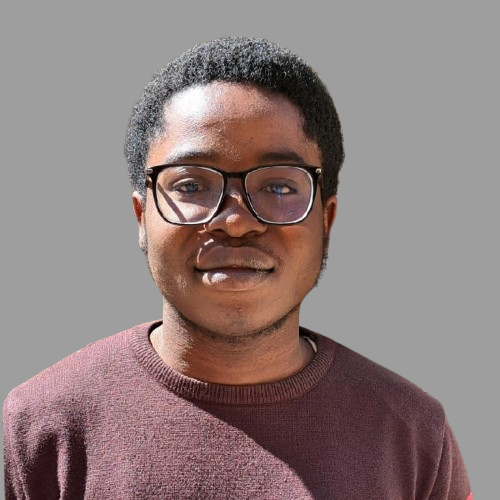
\includegraphics[width=2.35cm]{photo_richard.png}
\end{minipage}
\else
{\LARGE \textbf{Kossi Richard Allado}}\\
\textbf{Étudiant ingénieur en IA et cybersécurité | Machine Learning, Python, Data}\\
Beni Mellal, Maroc | +212 621 074 305 | \href{mailto:alladokossirichard2025@gmail.com}{alladokossirichard2025@gmail.com}\\
\href{https://allakori.github.io/}{allakori.github.io} | \href{https://github.com/ALLAKORI}{github.com/ALLAKORI} | \href{https://www.linkedin.com/in/kossi-richard-allado-50177b2a5}{linkedin.com/in/kossi-richard-allado}
\fi

\section{Profil}
Étudiant ingénieur en IA et cybersécurité à l'ENSA Beni Mellal, orienté machine learning appliqué, analyse de données, prototypage Python et IA générative locale. Portfolio GitHub avec maintenance prédictive, chatbot local, notebooks, interface desktop et documentation technique. Recherche un stage PFA IA/Data à partir de juillet 2026.

\section{Compétences techniques}
\textbf{Machine Learning / Data :} classification supervisée, Random Forest, préparation de données, évaluation, Jupyter.\\
\textbf{Python / Data stack :} Python, Pandas, Scikit-learn, SQL, Tkinter, ttkbootstrap, Git/GitHub.\\
\textbf{IA générative :} prompting, Chainlit, LangChain basics, CTransformers, modèles locaux, chatbot prototyping.\\
\textbf{Cybersécurité utile :} logs Linux/Windows, Splunk basics, IAM, Keycloak, cryptographie, réseau, CTF, Linux.

\section{Projets techniques}
\textbf{High-Pressure Pump Fault Prediction} \hfill Machine Learning / Maintenance prédictive\\
\href{https://github.com/ALLAKORI/Defaut-Pompe-Prediction}{github.com/ALLAKORI/Defaut-Pompe-Prediction}
\begin{itemize}
  \item Développé un prototype de maintenance prédictive pour pompe haute pression à partir de mesures capteurs : tension, puissance, vitesse, températures, pression et débit.
  \item Entraîné un modèle Random Forest avec Python, Pandas et Scikit-learn, puis créé une interface Tkinter/ttkbootstrap pour tester le niveau de risque.
\end{itemize}

\textbf{Local LLM and Chatbot Experiments} \hfill IA générative / Python\\
\href{https://github.com/ALLAKORI/MY-FIRST-AI-CHATBOT}{github.com/ALLAKORI/MY-FIRST-AI-CHATBOT}
\begin{itemize}
  \item Prototypé un chatbot local avec Python, Chainlit, LangChain basics, CTransformers et modèles GGUF.
  \item Testé prompting, logique conversationnelle et streaming pour mieux comprendre les limites des modèles locaux.
\end{itemize}

\textbf{Volt Typhoon Log Investigation} \hfill Data security / Analyse de logs\\
\href{https://allakori.github.io/writeups/tryhackme/volt-typhoon/}{allakori.github.io/writeups/tryhackme/volt-typhoon}
\begin{itemize}
  \item Analysé des logs Splunk pour reconstruire une intrusion sur 9 phases MITRE ATT\&CK et extraire 10+ indicateurs.
  \item Structuré les résultats dans un write-up technique avec requêtes, timeline, preuves et idées de détection.
\end{itemize}

\textbf{Portfolio GitHub IA et cybersécurité} \hfill Documentation / Preuve technique\\
\href{https://github.com/ALLAKORI}{github.com/ALLAKORI}
\begin{itemize}
  \item Organisé 22 dépôts GitHub autour de l'IA appliquée, des labs cybersécurité, des CTF et de la documentation technique.
  \item Présenté les projets sous forme de cas d'étude : objectif, outils, méthode, résultats, limites et prochaines améliorations.
\end{itemize}

\section{Expérience}
\role{Stagiaire IA / Maintenance prédictive}{ONEE - Branche Eau, Kasba Tadla}{Août 2025}
\begin{itemize}
  \item Préparé et analysé des données capteurs de pompe haute pression pour prédire des défauts potentiels.
  \item Construit un prototype Python combinant modèle Random Forest, pipeline de préparation de données et interface de test.
\end{itemize}

\section{Formation}
\edu{Cycle ingénieur}{Cybersécurité et Intelligence Artificielle, ENSA Beni Mellal}{2024 - Présent}{}
\edu{DEUST}{Mathématiques, Informatique, Physique, FST Fès}{2022 - 2024}{-- Mention Bien}
\edu{Baccalauréat scientifique}{Série D, Lycée de Djagblé, Togo}{2022}{-- Mention Très Bien}

\section{Certifications et réalisations}
IBM Introduction to Data Engineering | Cisco Ethical Hacker | Google Cybersecurity : Foundations et Play It Safe | Udemy Cryptography and Hashing | CSIA CTF 2026 : 1ère place

\section{Langues}
Français : courant | Anglais : professionnel technique | Éwé : langue maternelle

\end{document}
